\documentclass[A4paper,12pt]{article}

% --- Math & fonts ---
\usepackage[centertags]{amsmath}
\usepackage{amsfonts}
\usepackage{amssymb}
\usepackage{amsthm}
\usepackage{latexsym}
\usepackage{mathptmx}

% --- Graphics & figures ---
\usepackage{graphicx}
\usepackage{epsfig}
\usepackage{epstopdf}
\usepackage{float}
\usepackage{placeins}
\usepackage{caption}
\usepackage{adjustbox}
\usepackage{rotating}
\usepackage{lscape}

% --- Colors, frames & boxes ---
\usepackage[table,xcdraw]{xcolor}
\usepackage{framed}
\usepackage{fancybox}
\usepackage{color}

% --- Tables ---
\usepackage{booktabs}
\usepackage{threeparttable}

% --- Formatting ---
\usepackage{newlfont}
\usepackage{setspace}
\usepackage{kantlipsum}
\usepackage{fancyhdr}
\usepackage[normalem]{ulem}
\useunder{\uline}{\ul}{}

% --- Page layout ---
\usepackage[hmargin=1.4in,vmargin=1.4in]{geometry}

% --- References with natbib ---
\usepackage[numbers,sort&compress]{natbib}
\bibliographystyle{unsrt}


\setlength{\parindent}{0pt}
\setlength{\parskip}{1em} % adds vertical space between paragraphs

\newgeometry{left=1in,right=1.0in,top=1.0in,bottom=1in}
\setlength\extrarowheight{6.5pt}
%Created by Dr. M. Faisal Nadeem CUI Lahore
\pagestyle{fancy}
\fancyhf{}
%\cfoot{Page \thepage \hspace{1pt} of \pageref{LastPage}}
\renewcommand{\headrulewidth}{0pt}
\renewcommand*\FrameCommand{\hskip0.6cm\fcolorbox{black}{white}}%
\newlength{\framedline}
\setlength{\framedline}{0.966\textwidth}
\let\oldrule\rule
\renewcommand{\rule}[2]{
	\hspace*{-6.3pt}\oldrule{\framedline}{0.4pt}\newline}
 \linespread{1.213}


\begin{document}

\begin{center}

\textsc{\huge COMSATS University Islamabad \\[0.6cm]   Attock Campus}\\[0.6cm]


\includegraphics[height=3.5cm]{comsats.jpg}

\vspace{0.8cm}

{\LARGE \textbf{Project Proposal}}\\[0.8cm]

for\\[0.8cm]

{\LARGE Project Title}\\[0.8cm]

by\\[0.4cm]

STUDENT NAME 1 \\[0.2cm]
STUDENT NAME 2 \\[0.8cm]

CIIT/XXXX-XXX-XXX/ATK \\[0.2cm]
CIIT/XXXX-XXX-XXX/ATK \\[1.2cm]

\textbf{Supervisor}\\[0.4cm]
Write Supervisor Name Here\\[3cm]

\textbf{Bachelor of Science in Artificial Intelligence (2022–2026)}

\end{center}


\newpage
\begin{center}

\LARGE{Write your Project  Title here}\\
\vspace{0.5in}

\normalsize{By}\\
\vspace{0.5in}
\large{\textit{Write your Name Here}\\
{\textit{CIIT/FA23-RCS-000/ATK}}}\\
\large{\textit{Write your Name Here}\\
{\textit{CIIT/FA23-RCS-000/ATK}}}\\
\vspace{0.5in}

\normalsize{As the supervisor, I have reviewed the proposed project and found it to be feasible, relevant, and aligned with the academic and industry standards. I recommend this project for evaluation by the committee to assess its viability and approval for further development.}\\
\end{center}

\vspace{0.1in}

Supervisor Signature:\line(1,0){280}
\begin{center}
\normalsize{Supervisor Name\\
Department of Computer Science, (CUI) Attock Campus}
\end{center}
\vspace{0.1in}
\newpage

\pagenumbering{gobble}
%\renewcommand{\maketitle}{%

\cfoot{\thepage}
\vspace{0in}
\pagenumbering{arabic}
\medskip

\section*{\fontsize{16}{12}\selectfont  Project Summary}
It  is a  summary  of  the  research  work  presented  in  the  synopsis.  There  should not be any citations in the summary. It should not be more than half a page (MAX 300 Words). It should embrace the following principal areas: (i) The rationale of the study; (ii) Broader challenges of the research area; (iii) Already developed solutions (iv) Research Gaps; (v) Problem formulation (vi) Objective of the current/proposed study; (vii) Broader methodology to be embraced; (vii) significance of the proposed work.
[\textcolor{red}{Introduction must start from next page. remove this line before submiting the final document} ]
\pagestyle{fancy}

\newpage
\section{ Introduction}
In recent years, humanoid robotics has seen significant advancements, with artificial intelligence (AI) 
playing a crucial role in enhancing human-robot interactions. The primary objective behind humanoid 
robots is to create a seamless communication bridge between humans and machines, allowing robots to 
respond naturally to human presence through speech, gestures and expressions. Various industries, such as 
customer service, education and healthcare, have begun integrating humanoid robots to assist in daily 
operations. However, most existing humanoid robots are either too expensive, highly complex, or designed \cite{r1}
for industrial applications, making them inaccessible for personalized, small-scale human interaction 
\newline
\begin{figure}[h]
    \centering
    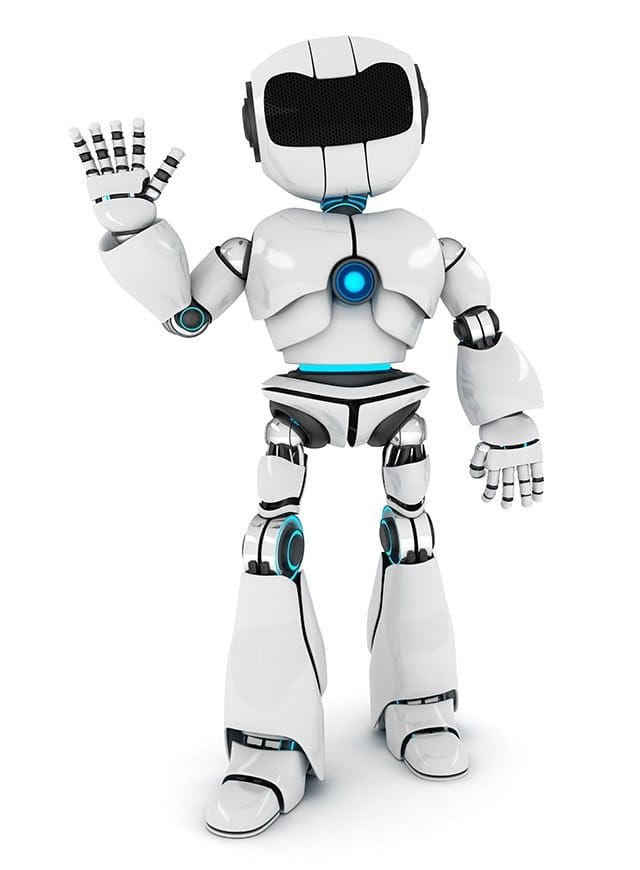
\includegraphics[width=4cm]{robot.jpg}
    \caption{}
    \label{fig:galaxy}
\end{figure}
\newline
\newline
This project aims to develop a compact, interactive humanoid robot designed to remain stationary on a 
table while engaging in intelligent, human-like communication. The robot will be equipped with 
advanced camera sensors embedded in its eyes to detect human presence and initiate interaction. As soon 
as an individual approaches, the robot will capture their image in real time for facial recognition. If the person is identified in its trained database, it will display a 
welcoming green expression on its embedded LED screen and greet them by name, saying, " Welcome 
back, [Person’s Name]. It is a pleasure to see you. I [Robot’s name] am an intelligent humanoid assistant 
designed to interact, assist, and enhance user experiences. My capabilities include [list of features], and I 
can perform [list of abilities]. How may I assist you today? " This interaction will seamlessly transition 
into a Q&A session, where the individual can ask questions, and the robot will respond with well
structured, meaningful answers while maintaining synchronized speech and gestures. Natural movements, 
such as hand gestures, head tilts, and blinking, will further enhance the engagement, making the 
conversation feel more interactive and lifelike.
\newline
\newline
From a different perspective, If the robot does not recognize the individual and determines that their face is 
not in the trained database, it will display a curious red expression on its LED screen and politely request 
authentication. It will state, " I do not seem to have your details in my memory. Would you like me to 
register your face  for a more personalized experience in the future ? " Upon receiving consent, the robot 
will capture the individual’s image and confirm the registration by conveying, " Your facial data has been 
successfully recorded. The next time you visit, I will recognize and greet you accordingly. For now, please 
introduce yourself by stating your name. " Once the person provides their name, the robot will proceed 
with its introduction before initiating the Q&A session. Throughout the conversation, synchronized speech 
and gestures will ensure a fluid and engaging experience to maintain realism. At the conclusion of the 
dialogue exchange round, upon receiving an audio command such as " Please provide your closing 
statement, " the robot will gracefully respond, " It has been a pleasure interacting with you. I am 
continuously evolving and improving to better assist you. Thank you for your time, and I look forward to 
our next conversation " 
\newline
\newline
In summary, this project focuses on developing a stationary, cost-effective, and interactive humanoid robot 
capable of engaging in personalized conversations using facial recognition, speech synchronization, and 
expressive gestures. Unlike traditional humanoid robots that prioritize physical movement, this project 
emphasizes human-like interaction through intelligent responses and synchronized actions. By integrating 
AI, computer vision, and robotics principles, this robot serves as a practical and scalable model for 
educational, social, and commercial applications.
\newline
\newline
[\textcolor{red}{Introduction length is not specific write introduction as much needed for your project also remove this line before submiting the final document} ]

\section {Literature Review}
This paper \cite{r1} an efficient CNN-based framework for face recognition and tracking in unconstrained environments. Implemented as a modular ROS package, it enhances HRI applications by improving real-time recognition across varying conditions.\newline

This study \cite{r2} presents a real-time system for human face tracking and recognition under varying conditions, including different facial expressions, poses, and dynamic backgrounds. The system utilizes the Viola-Jones algorithm for face detection and the Principal Component Analysis (PCA) method for recognition, achieving a recognition rate of 91.12\%. \newline

ExGenNet is a deep generative model that enables humanoid robots to display lifelike facial expressions \cite{r3}. Evaluated on Furhat and Elenoide robots, it successfully generated recognizable expressions, verified through user studies.\newline

This paper \cite{r4} explores improvements in vision and voice recognition for humanoid robots, enhancing their ability to interact with humans. It highlights AI-driven computer vision for real-time face, gesture, and object detection, along with advancements in natural language processing (NLP) to improve speech recognition and conversational abilities. The integration of multi-modal perception systems, including auditory and tactile sensing, allows robots to better understand their environment. These advancements aim to make humanoid robots more responsive, adaptive, and suitable for real-world applications.\newline

Nadine is a humanoid social robot \cite{r5} designed to exhibit human-like behaviors, including facial recognition, emotion detection, and gesture-based interactions. Equipped with 3D depth cameras, webcams, and microphones, Nadine can perceive and respond to users' emotions and gestures, facilitating natural human-robot interactions. \newline

\begin{table}[h!] 
    \centering 
    \caption{Related System Analysis with proposed project solution} 
    \label{tab:sample} 
    \begin{tabular}{|p{0.3\textwidth}|p{0.3\textwidth}|p{0.3\textwidth}|} \hline \textbf{Application Name} & \textbf{Weakness} & \textbf{Proposed Project Solu tion} 
    \\ \hline
    Row 1, Cell 1 & Row 1, Cell 2 & Row 1, Cell 3 \\ 
    \hline Row 2, Cell 1 & Row 2, Cell 2 & Row 2, Cell 3 \\ 
    \hline Row 3, Cell 1 & Row 3, Cell 2 & Row 3, Cell 3 \\ 
    \hline Row 4, Cell 1 & Row 4, Cell 2 & Row 4, Cell 3 \\ 
    \hline Row 5, Cell 1 & Row 5, Cell 2 & Row 5, Cell 3 \\
    \hline 
    \end{tabular} 
\end{table}

\section {Problem Statement}
The increasing impact of human activities on the environment has led to significant challenges such as climate change, deforestation, and pollution. These issues threaten ecosystems, biodiversity, and the well-being of future generations. Despite growing awareness, many industries and communities continue to rely on unsustainable practices due to a lack of accessible alternatives or economic constraints. This project seeks to address these challenges by developing innovative, sustainable solutions that balance environmental preservation with economic and social needs. By focusing on [specific issue, e.g., renewable energy, waste management, or conservation], the project aims to contribute to a more sustainable future.

\section{ Proposed Solution}
Write proposed solution of your project  here....

\begin{itemize}
    \item Write solution  here in bullet points. write seprate solution in seprate bullet point . 
\end{itemize}

\section { Vision Statement}
Vision of your project


\section { Scope}
Write Scope of your project


\section {Methodology}
This section provides insight on what methodology you will employ in the development of the envisioned system. It is the systematic, theoretical analysis of the methods applied to your of study. It can comprise of step by step procedures, flowcharts, block diagrams or algorithms of the proposed system.

\begin{figure}[hh]
    \centering
    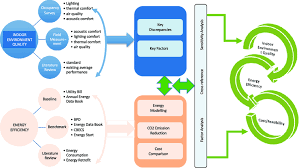
\includegraphics[width=0.9\linewidth]{download.png}
    \caption{Caption}
    \label{fig:enter-label}
\end{figure}

\section { Tools and Technologies}

Following is the sample research design for reference and is not exhaustive

\section { Applications of this Project}

This project has a wide range of applications, including : 


\begin{itemize}
    \item write here applications of your project. 
    \item write here applications of your project. 
    \item write here applications of your project. 
    \item write here applications of your project. 
\end{itemize}

\section {	WBS and Gantt Chart}

Following is the sample research design for reference and is not exhaustive.
\begin{figure}[hh]
    \centering
    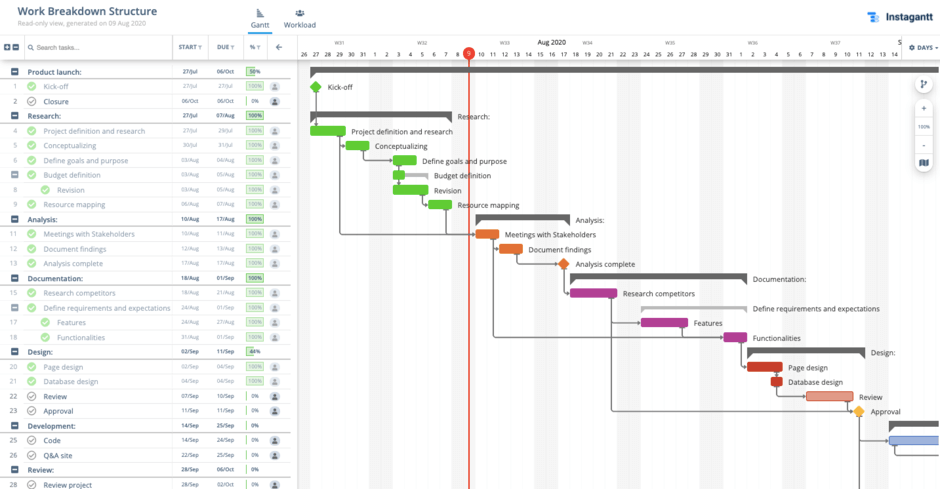
\includegraphics[width=0.9\linewidth]{wbs.png}
    \caption{Caption}
    \label{fig:enter-label}
\end{figure}

\section {Mockups}

Following is the sample research design for reference and is not exhaustive

\begin{figure}[h]
    \centering
    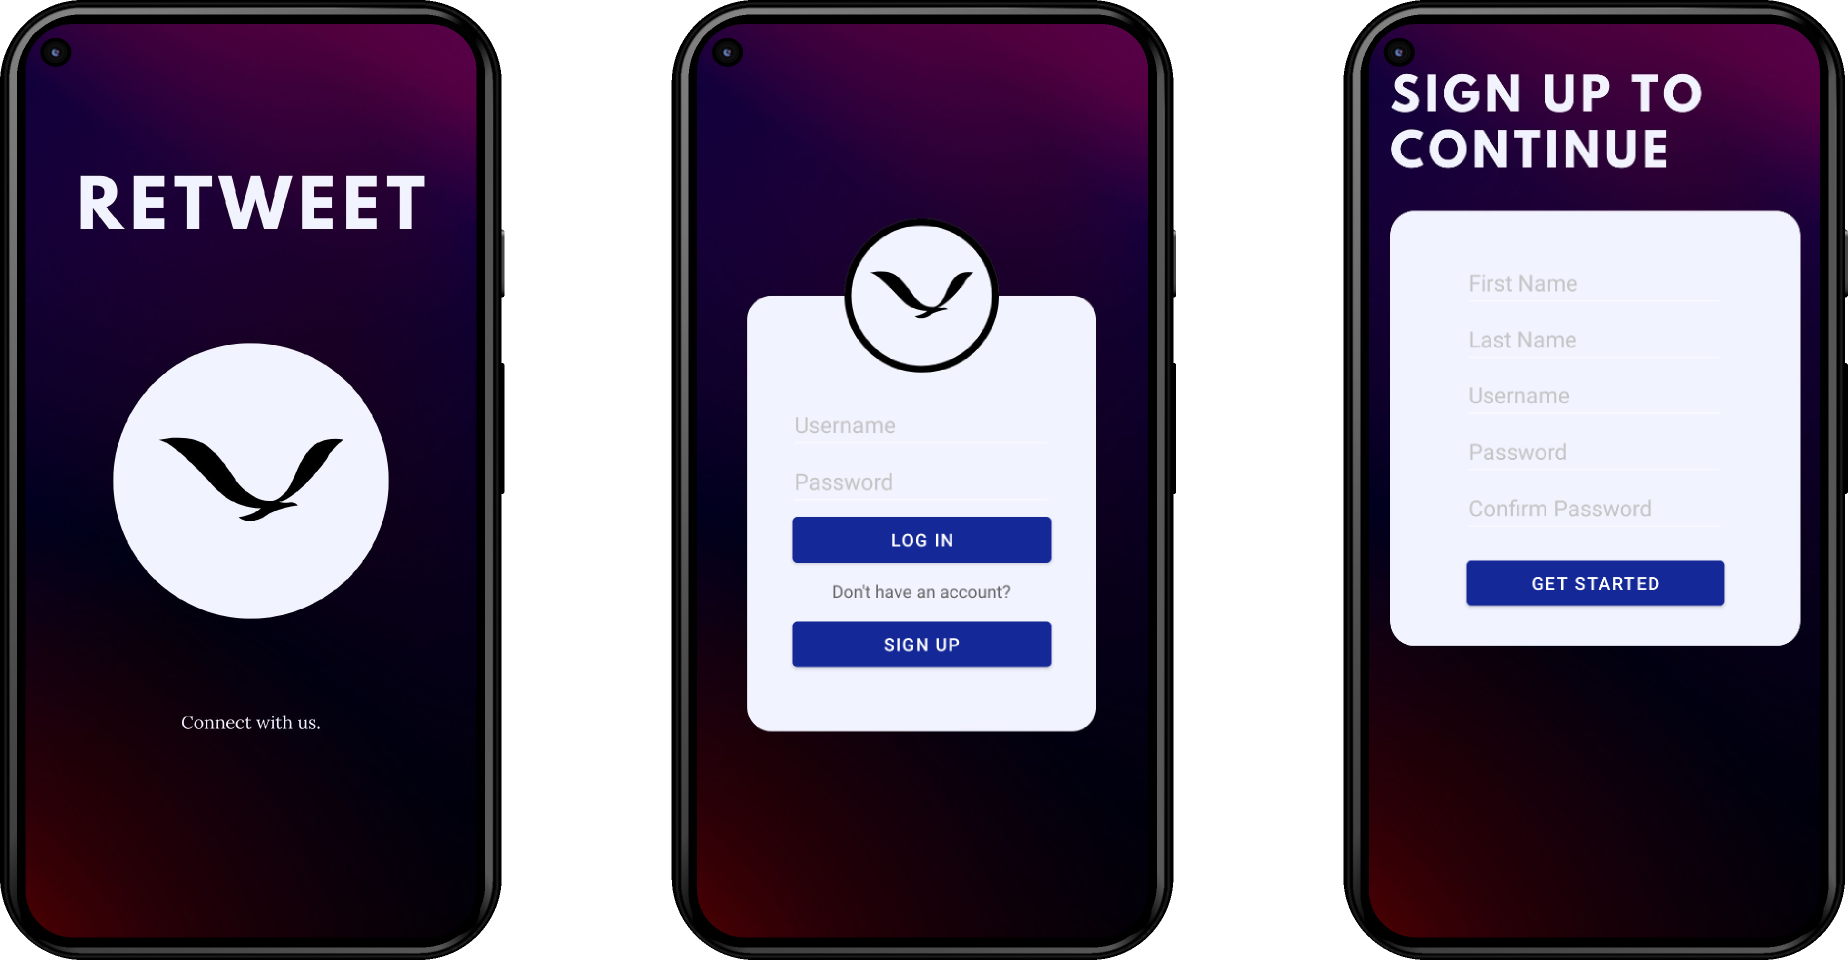
\includegraphics[width=14cm,height=7.5cm]{downlaod2.png}
    \caption{}
    \label{fig:galaxy}
\end{figure}
\newpage
\bibliography{final}
\newpage
\end{document}
